\begin{song}{O malém rytíři}{D}{Traband}

\begin{SBChorus}

Ref: \Ch{hmi}{Jede} jede rytíř, \Ch{D}{jede} do kraje

\Ch{A}{Nové dobrodružství} \Ch{hmi}{v dálce} hledaje

\Ch{hmi}{Neví} co je bázeň, \Ch{D}{neví} co je strach

\Ch{A}{Má} jen velké srdce \Ch{hmi}{a na} botách prach

\end{SBChorus}

\begin{SBVerse}

\Ch{G}{Jednou} takhle v neděli, \Ch{F#}{slunce} pěkně hřálo

\Ch{G}{Bylo} kolem poledne, \Ch{F#}{když} tu se to stalo

\Ch{G}{Panáček} uhodí \Ch{A}{pěstičkou} do stolu:

\Ch{G}{Dosti }bylo pohodlí \Ch{A}{a }plnejch kastrólů!

\Ch{hmi}{Ještě} dneska stůjcostůj \Ch{A}{musím} na cestu se dát

\Ch{G}{Tak} zavolejte sloužící a \Ch{F#}{dejte} koně osedlat!

\end{SBVerse}

\begin{SBVerse}

Ale milostpane! spráskne ruce starý čeledín

Ale pán už sedí v sedle a volá s nadšením:

Má povinnost mi velí pomáhat potřebným

Ochraňovat chudé, slabé, léčit rány nemocným

Marně za ním volá stará hospodyně:

Vraťte se pane, lidi sou svině!

\end{SBVerse}

\begin{SBVerse}

Ale sotva dojel kousek za městskou bránu

Z lesa na něj vyskočila banda trhanů

Všichni ti chudí, slabí, potřební - no chátra špinavá

Vrhli se na něj a bili ho hlava nehlava

Než se stačil vzpamatovat, bylo málem po něm

Ukradli mu co kde měl a sežrali mu koně

\end{SBVerse}

\begin{SBVerse}

Vzhůru srdce! zvolá rytíř, nekončí má pouť

Svou čest a slávu dobudu, jen z cesty neuhnout!

Hle, můj meč! (a zvedl ze země kus drátu)

A zde můj štít a přílbice! (plechovka od špenátu)

Pak osedlal si pavouka, sed na něj, řekl Hyjé!

Jedem vysvobodit princeznu z letargie

\end{SBVerse}

\begin{SBVerse}

A šíleně smutná princezna sotva ho viděla

Vyprskla smíchy a plácla se do čela

Začala se chechtat, až jí z očí tekly slzy

To je neskutečný, volala, jak jsou dneska lidi drzý!

O mou ruku se chce ucházet tahle figůra

Hej, zbrojnoši, ukažte mu rychle cestu ze dvora!

\end{SBVerse}

\begin{SBVerse}

Tak jede malý rytíř svojí cestou dál

Hlavu hrdě vzhůru - on svou bitvu neprohrál

I když král ho nechal vypráskat a drak mu sežral boty

A děvka z ulice mu plivla na kalhoty

Ve světě kde jsou lidi na lidi jak vlci

Zůstává rytířem - ve svém srdci

\end{SBVerse}
\begin{center}
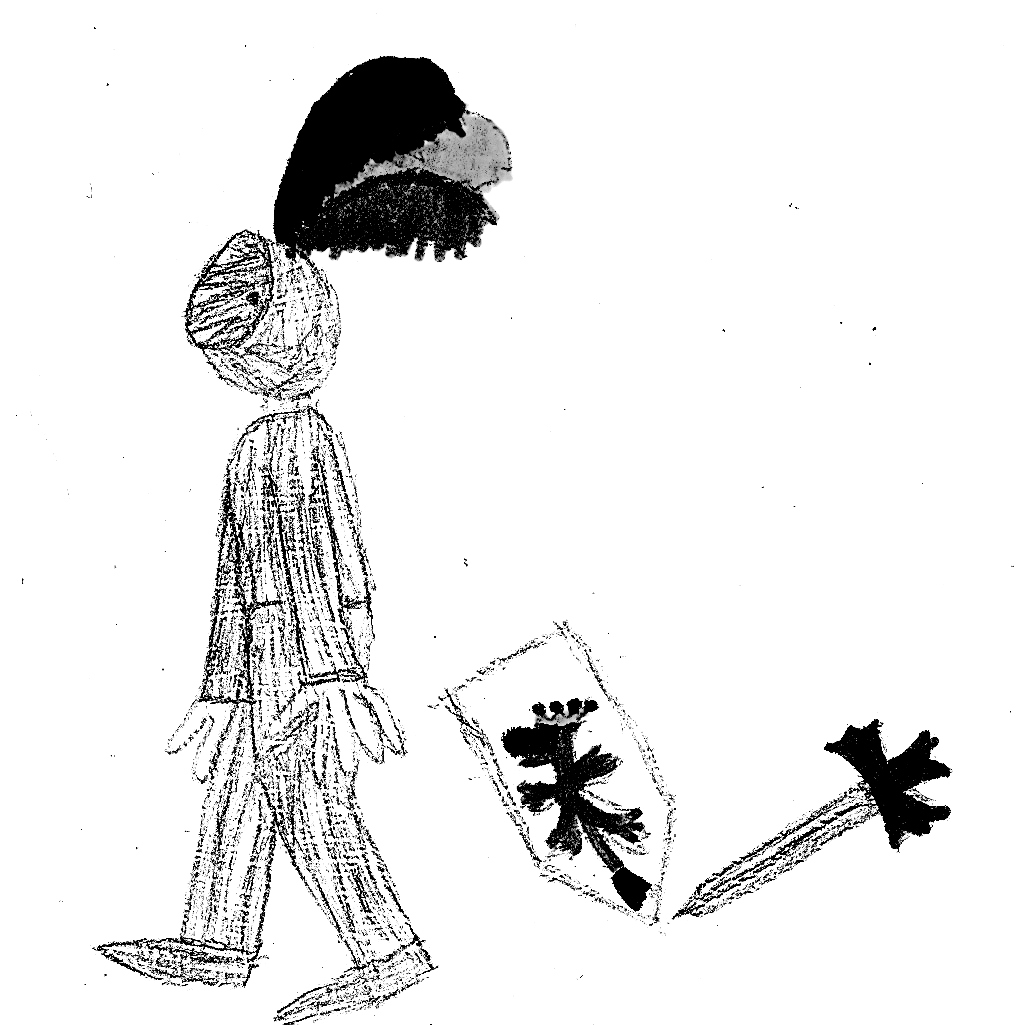
\includegraphics[width=6cm]{pict/asi-rytíř.jpg}
\end{center}
\end{song}

\pagebreak